\section{Implementation}
In this section, we will describe the implementation of the timed automaton model from the previous section, shown in Figure \ref{fig:automaton}. Our tool of choice is UPPAAL, an integrated solution for modeling, simulation, and verification of timed automata. We will present the implementation details and limitations imposed on the model in the following subsection.  Model variables representing its state will be described along with the most important functions.


\subsection{Model}
The implementation of the timed automaton, shown in Figure \ref{fig:implementation}, includes an additional state called \texttt{grid}, which is not present in the automaton depicted in Figure \ref{fig:automaton}. Global functions of the implementation abstract away the underlying complexity. The  \texttt{grid} state is a consequence of imposing limitations on the environment size defined in the previous section. This allows us to reduce the state space size and perform verification. It is the biggest change made to the original algorithm, defined in Figure \ref{fig:pseudocode}. In that state, it is determined whether a robot has reached the boundary of the grid. If yes, the robot will transition to the state \texttt{turn\_180} and change its direction by 180 degrees as it cannot continue moving forward outside of its environment. If a robot has not reached the boundary of its environment it will transition to the \texttt{if} state where it will transition to further states based on the original rules of the algorithm.

\begin{figure}[H]
\caption{Asynchronous implementation of the Beta algorithm}
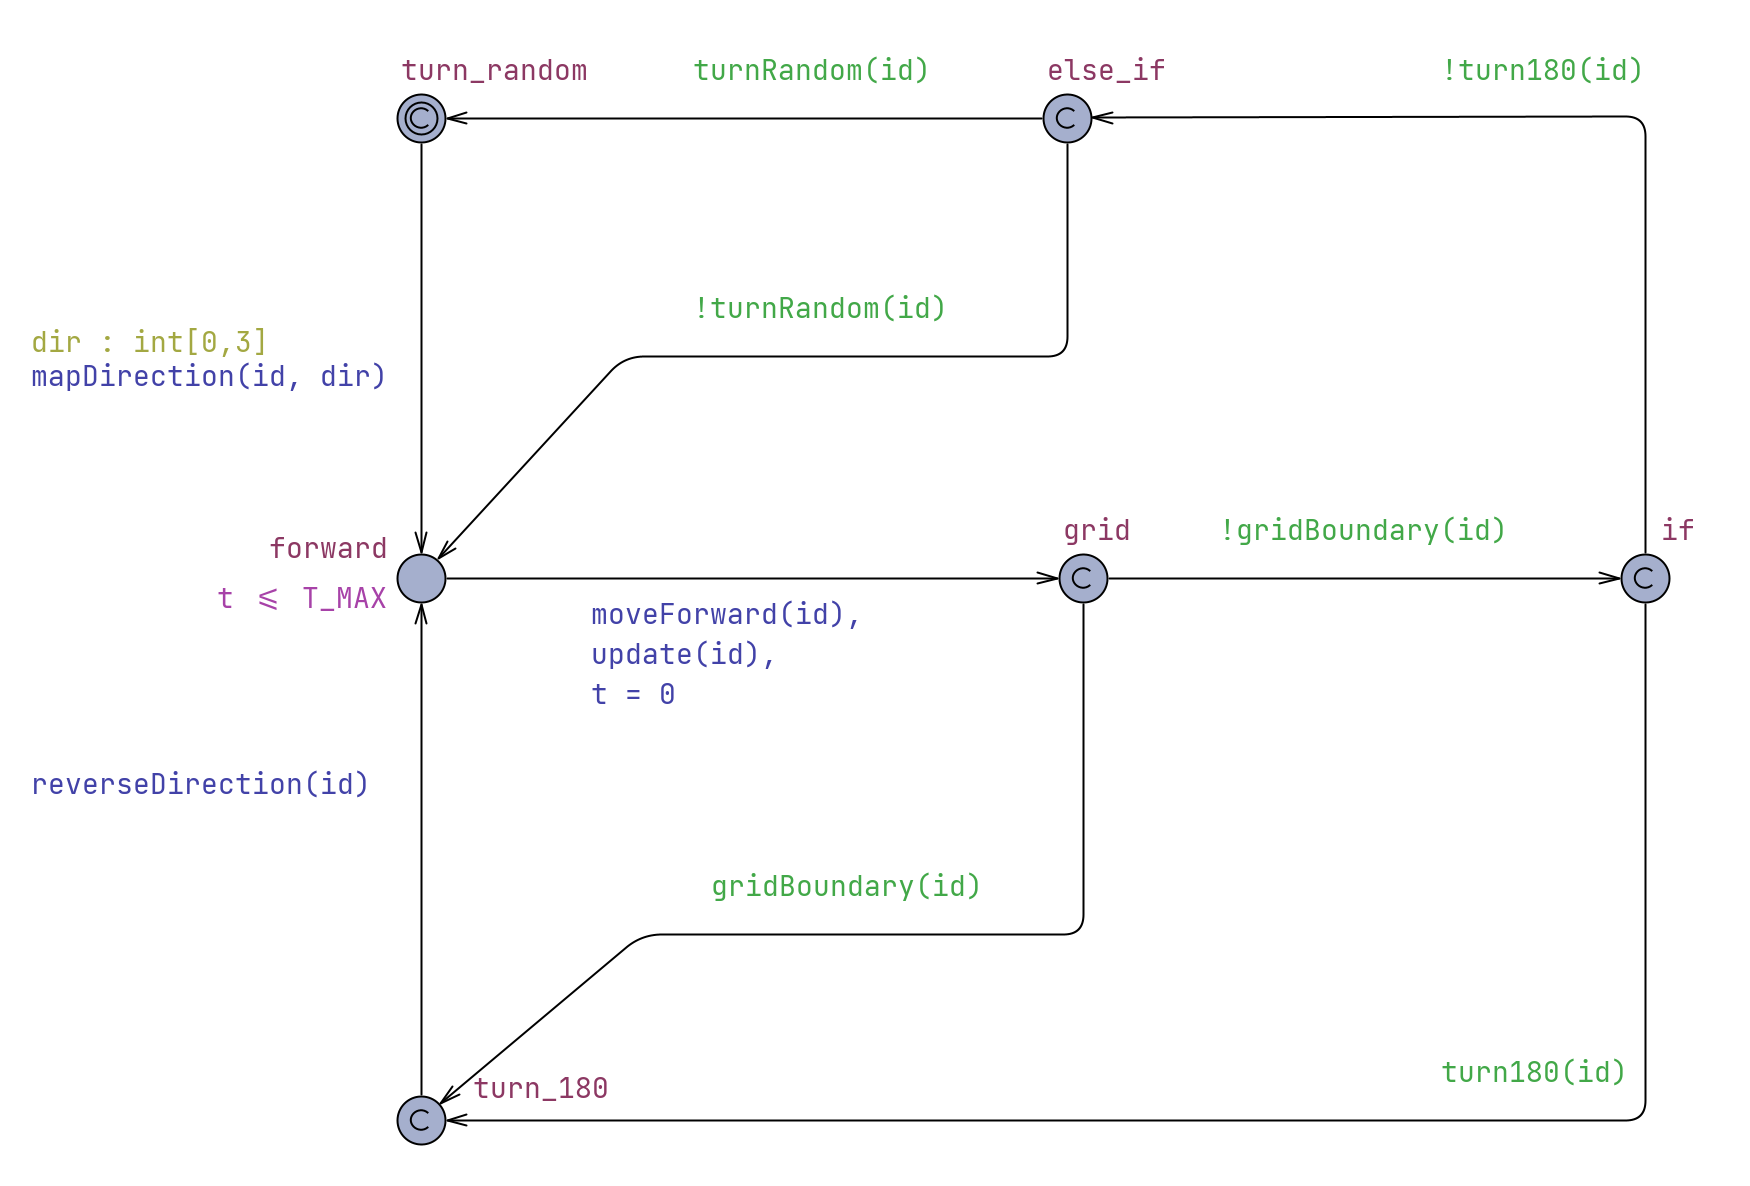
\includegraphics[width=\textwidth]{images/implementation_asynchronous.png}
\label{fig:implementation}
\end{figure}

\noindent
The implementation of the Beta algorithm presented in Figure \ref{fig:implementation} is asynchronous as stated by the author of the algorithm. Robots can move at different pace and time, independent of each other. We also implemented a synchronized version of the Beta algorithm to investigate the influence of the concurrency mode on verification results. The synchronized implementation is presented in Figure \ref{fig:implementation_synchronised}, and its synchronization mechanism in Figure \ref{fig:implementation_synchronised_barrier}. The synchronized version enforces that all robots move at the same time. The synchronization mechanism, which we will call barrier, has a variable \texttt{n} initialized to the number of robots in the swarm. Each time a robot transitions to the \texttt{forward} state it will use a synchronization channel \texttt{done} to notify the barrier. The barrier will decrement its variable \texttt{n} upon receiving a signal from a robot. When the value of \texttt{n} reaches 0, all robots will be blocked in the \texttt{forward} state. The barrier then will send a signal using synchronization channel \texttt{step} and reset the value of the variable \texttt{n} to the number of robots in the swarm. Robots waiting in the \texttt{forward} state will receive this signal from the \texttt{step} channel and transition to \texttt{grid} state at the same time. They will then progress to the \texttt{forward} state in the random order, possibly changing its direction. The order in which they reach the \texttt{forward} state does not influence swarm behavior. A robot decides whether to change direction based on the state of the swarm. The state of the swarm, most importantly robot positions, will not change until the next collective step forward. In other words, the direction of the robot is not a variable that influences the behavior of another robot, unlike its position. 

\begin{figure}[H]
\caption{Synchronised implementation of the Beta algorithm}
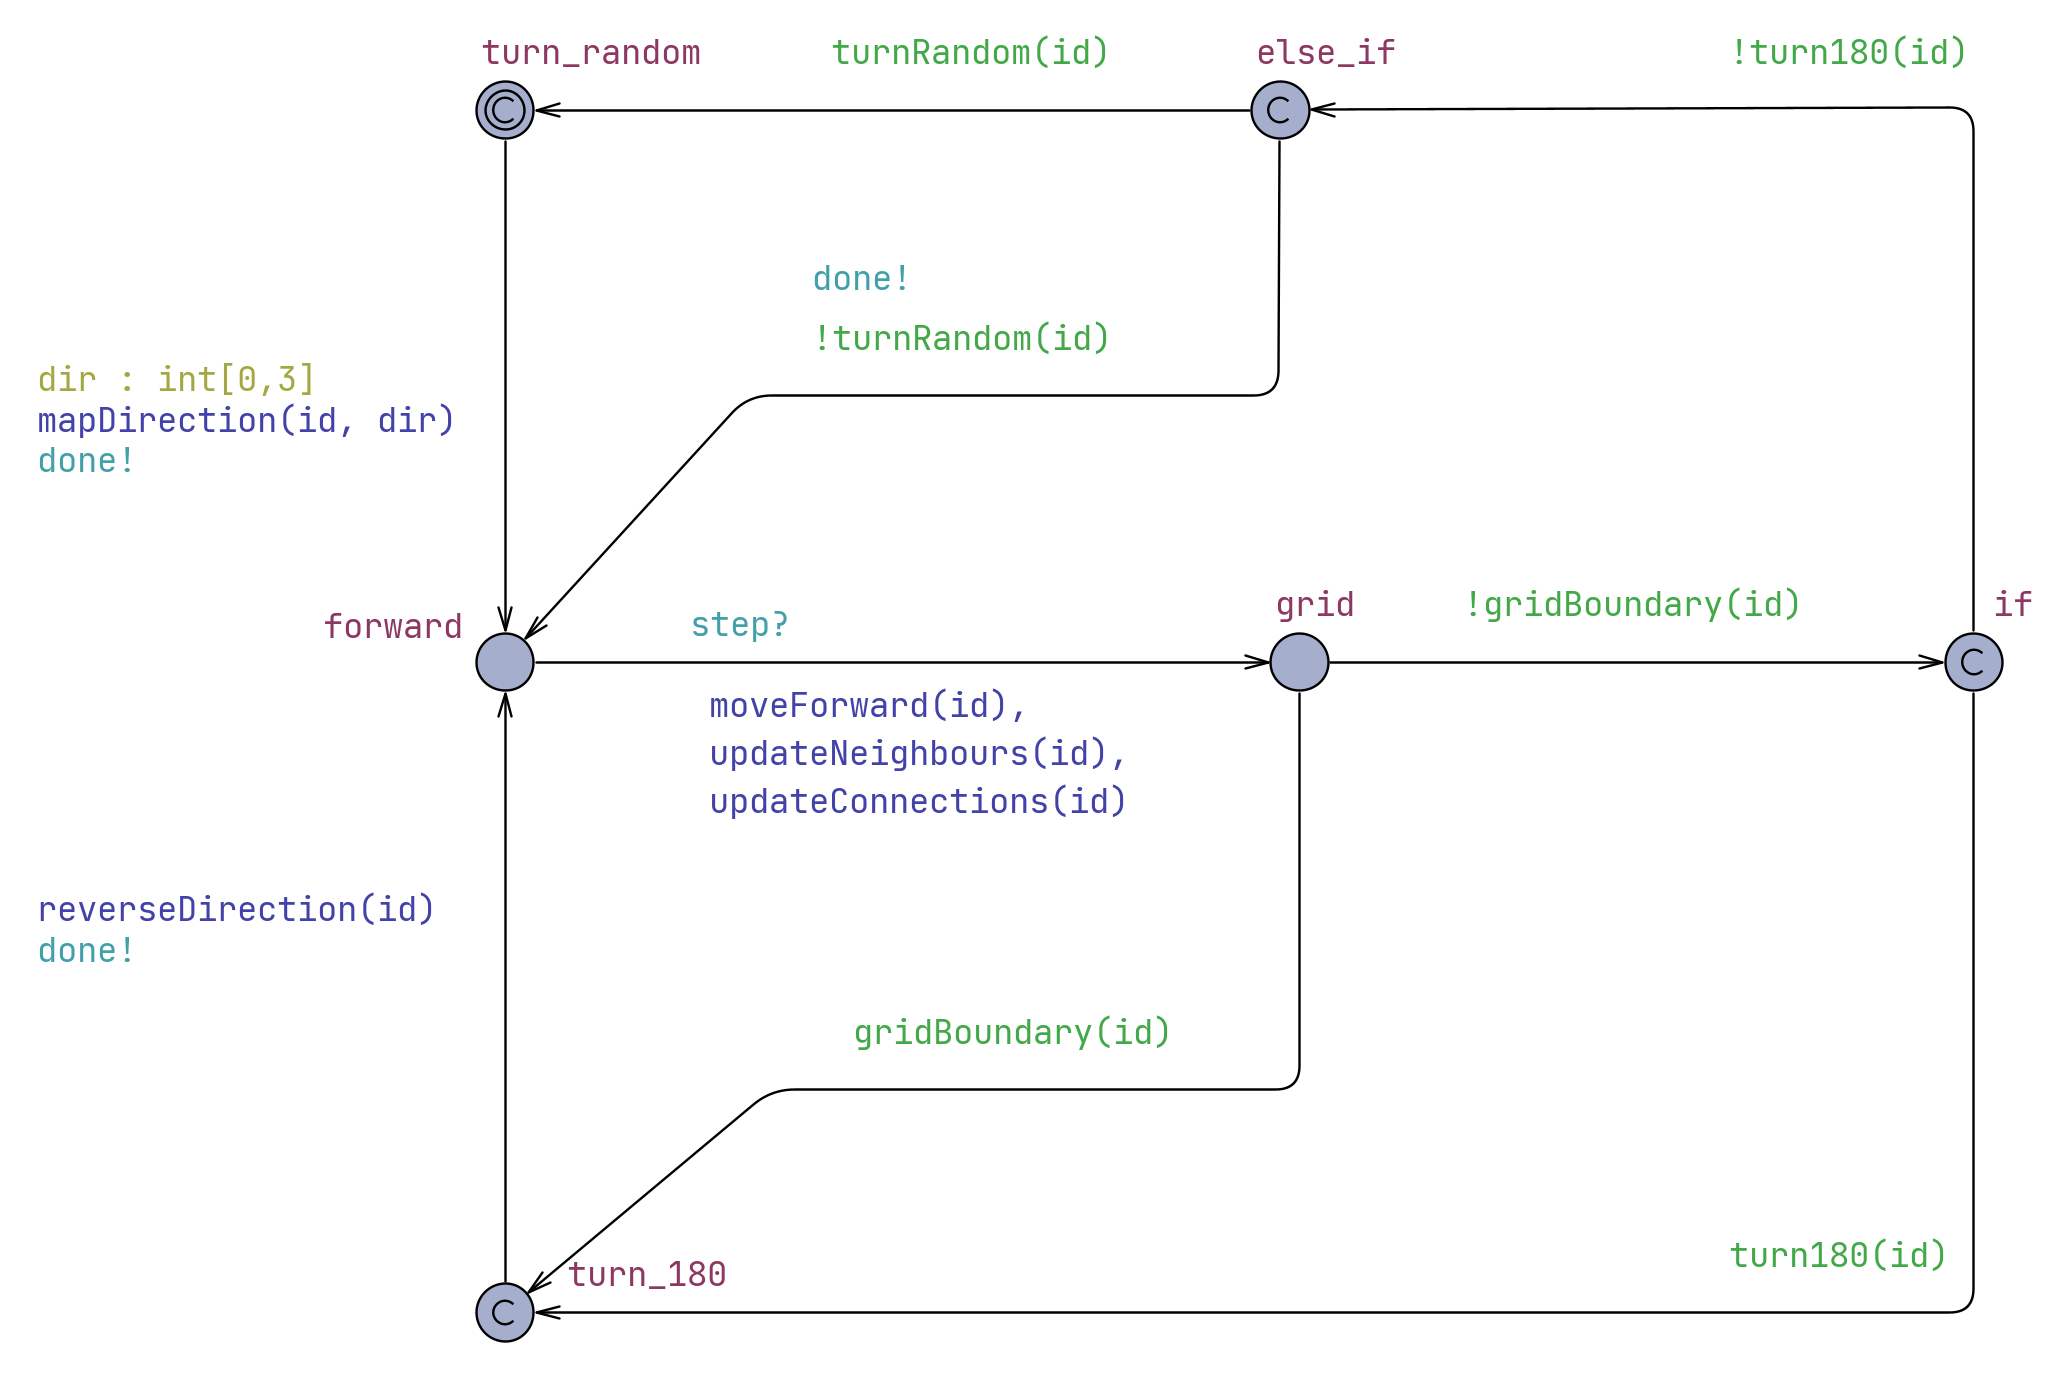
\includegraphics[width=\textwidth]{images/implementation_synchronised.png}
\label{fig:implementation_synchronised}
\end{figure}

\begin{figure}[H]
\caption{Synchronisation mechanism}
\centering
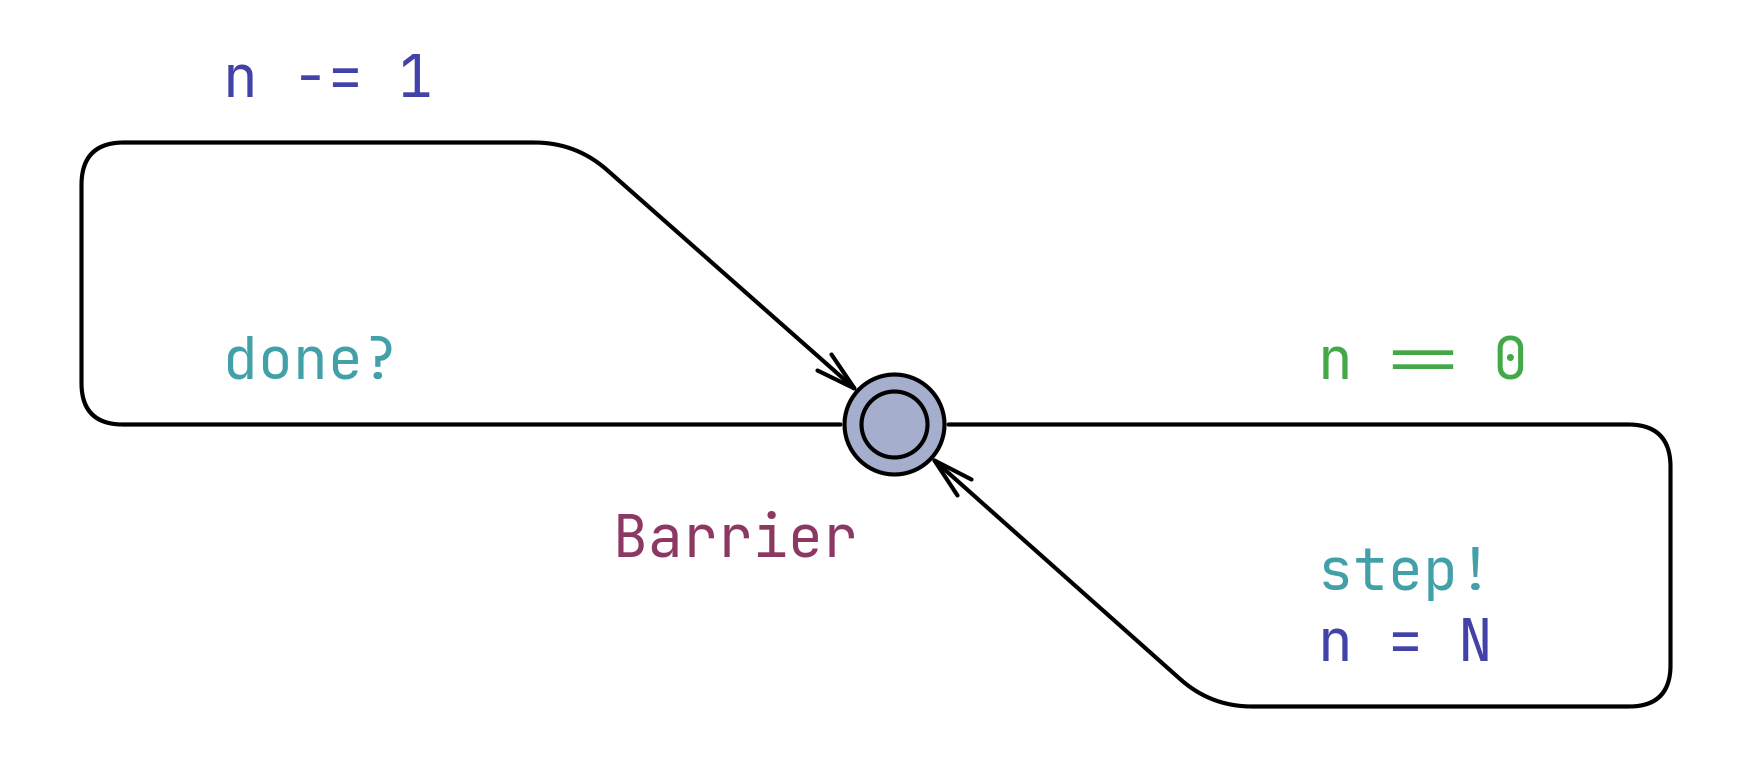
\includegraphics[width=0.5\textwidth]{images/implementation_synchronised_barrier.png}
\label{fig:implementation_synchronised_barrier}
\end{figure}

\subsection{Movement}
Before explaining the functions that control the movement and direction of the robot, we will first introduce the data structures used by these functions.
\\\\
\texttt{x[N]} - list of x-axis coordinates for each robot;\\
\texttt{y[N]} - list of y-axis coordinates for each robot;\\
\texttt{x\_dir[N]} - list of x-axis directions for each robot;\\
\texttt{y\_dir[N]} - list of y-axis directions for each robot;\\
\texttt{STEP} - step size, uniform for all robots;\\\\
\noindent
Three global functions govern the movement of the robot, namely, \texttt{mapDirection}, \texttt{reverseDirection}, \texttt{moveForward}. The \texttt{mapDirection} function is triggered upon transition from state \texttt{turn\_random} to state \texttt{forward} and provided with \texttt{id} of the robot and randomly drawn integer \texttt{dir} that will be mapped to one of four directions. The \texttt{reverseDirection} function is triggered upon transition from state \texttt{turn\_180} to state \texttt{forward} and provided with \texttt{id} of the robot whose direction is to be reversed. The \texttt{moveForward} function is triggered upon transition from state \texttt{forward} to state \texttt{grid} and provided with \texttt{id} of the robot that is to be moved forward. The implementation of those functions is shown in Figure \ref{fig:movement_implementation}.

\begin{figure}
\caption{Implementation of functions controlling robot movement}
\begin{lstlisting}[style=code]
void mapDirection(int id, int dir){
    if (dir == 0){
		// up
        x_dir[id] = 0;
        y_dir[id] = 1;
    }
    if (dir == 1){
		// right
        x_dir[id] = 1;
        y_dir[id] = 0;
    }
    if (dir == 2){
		// down
        x_dir[id] = 0;
        y_dir[id] = -1;
    }
    if (dir == 3){
		// left
        x_dir[id] = -1;
        y_dir[id] = 0;
    }
}

void reverseDirection(int id){
	x_dir[id] *= -1;
	y_dir[id] *= -1;
}

void moveForward(int id){
	x[id] += x_dir[id] * STEP;
	y[id] += y_dir[id] * STEP;
}
\end{lstlisting}
\label{fig:movement_implementation}
\end{figure}



\subsection{Connection}



\subsection{System variables}
